\chapter{Model 1: Linear Regression with Outlier Removal}\label{ch:model1}

% Include the dynamic values from model calibration
% Model 1 Calibrated Values
% Generated: 2025-10-02 01:58:23.185499
% Model: Linear with Outlier Removal

% Core Metrics
\renewcommand{\ModelOneRSquaredTrain}{0.2383}
\renewcommand{\ModelOneRSquaredTest}{0.2178}
\renewcommand{\ModelOneRMSETrain}{39,238}
\renewcommand{\ModelOneRMSETest}{39,500}
\renewcommand{\ModelOneMAETrain}{27,831}
\renewcommand{\ModelOneMAETest}{27,912}
\renewcommand{\ModelOneMAPETrain}{85.2}
\renewcommand{\ModelOneMAPETest}{84.8}
\renewcommand{\ModelOneCVMean}{0.2372}
\renewcommand{\ModelOneCVStd}{0.0196}
\renewcommand{\ModelOneWithinOneK}{2.4}
\renewcommand{\ModelOneWithinTwoK}{4.9}
\renewcommand{\ModelOneWithinFiveK}{15.8}
\renewcommand{\ModelOneWithinTenK}{28.5}
\renewcommand{\ModelOneWithinTwentyK}{49.5}
\renewcommand{\ModelOneTrainingSamples}{27,339}
\renewcommand{\ModelOneTestSamples}{6,834}

% Subgroup Metrics
\renewcommand{\ModelOneSubgrouplivingFHN}{5,941}
\renewcommand{\ModelOneSubgrouplivingFHRSquared}{0.222}
\renewcommand{\ModelOneSubgrouplivingFHRMSE}{39,928}
\renewcommand{\ModelOneSubgrouplivingFHBias}{-7,487}
\renewcommand{\ModelOneSubgrouplivingILSLN}{893}
\renewcommand{\ModelOneSubgrouplivingILSLRSquared}{0.179}
\renewcommand{\ModelOneSubgrouplivingILSLRMSE}{36,524}
\renewcommand{\ModelOneSubgrouplivingILSLBias}{-3,272}
\renewcommand{\ModelOneSubgroupageAgeUnderTwentyOneN}{694}
\renewcommand{\ModelOneSubgroupageAgeUnderTwentyOneRSquared}{0.138}
\renewcommand{\ModelOneSubgroupageAgeUnderTwentyOneRMSE}{34,649}
\renewcommand{\ModelOneSubgroupageAgeUnderTwentyOneBias}{-8,152}
\renewcommand{\ModelOneSubgroupageAgeTwentyOneToThirtyN}{1,797}
\renewcommand{\ModelOneSubgroupageAgeTwentyOneToThirtyRSquared}{0.161}
\renewcommand{\ModelOneSubgroupageAgeTwentyOneToThirtyRMSE}{44,751}
\renewcommand{\ModelOneSubgroupageAgeTwentyOneToThirtyBias}{-7,785}
\renewcommand{\ModelOneSubgroupageAgeThirtyOnePlusN}{4,343}
\renewcommand{\ModelOneSubgroupageAgeThirtyOnePlusRSquared}{0.218}
\renewcommand{\ModelOneSubgroupageAgeThirtyOnePlusRMSE}{37,876}
\renewcommand{\ModelOneSubgroupageAgeThirtyOnePlusBias}{-6,391}
\renewcommand{\ModelOneSubgroupcostQOneLowN}{1,709}
\renewcommand{\ModelOneSubgroupcostQOneLowRSquared}{-10.000}
\renewcommand{\ModelOneSubgroupcostQOneLowRMSE}{31,272}
\renewcommand{\ModelOneSubgroupcostQOneLowBias}{+24,162}
\renewcommand{\ModelOneSubgroupcostQTwoN}{1,708}
\renewcommand{\ModelOneSubgroupcostQTwoRSquared}{-6.029}
\renewcommand{\ModelOneSubgroupcostQTwoRMSE}{20,461}
\renewcommand{\ModelOneSubgroupcostQTwoBias}{+9,755}
\renewcommand{\ModelOneSubgroupcostQThreeN}{1,708}
\renewcommand{\ModelOneSubgroupcostQThreeRSquared}{-4.117}
\renewcommand{\ModelOneSubgroupcostQThreeRMSE}{26,401}
\renewcommand{\ModelOneSubgroupcostQThreeBias}{-13,739}
\renewcommand{\ModelOneSubgroupcostQFourHighN}{1,709}
\renewcommand{\ModelOneSubgroupcostQFourHighRSquared}{-2.230}
\renewcommand{\ModelOneSubgroupcostQFourHighRMSE}{64,390}
\renewcommand{\ModelOneSubgroupcostQFourHighBias}{-47,917}

% Variance Metrics
\renewcommand{\ModelOneCVActual}{1.010}
\renewcommand{\ModelOneCVPredicted}{0.692}
\renewcommand{\ModelOnePredictionInterval}{152,432}
\renewcommand{\ModelOneBudgetActualCorr}{0.498}
\renewcommand{\ModelOneQuarterlyVariance}{87.9}
\renewcommand{\ModelOneAnnualAdjustmentRate}{92.4}

% Population Scenarios
\renewcommand{\ModelOnePopcurrentbaselineClients}{32,188}
\renewcommand{\ModelOnePopcurrentbaselineAvgAlloc}{37,280}
\renewcommand{\ModelOnePopcurrentbaselineWaitlistChange}{+0}
\renewcommand{\ModelOnePopcurrentbaselineWaitlistPct}{+0.0}
\renewcommand{\ModelOnePopmodelbalancedClients}{32,831}
\renewcommand{\ModelOnePopmodelbalancedAvgAlloc}{36,534}
\renewcommand{\ModelOnePopmodelbalancedWaitlistChange}{+643}
\renewcommand{\ModelOnePopmodelbalancedWaitlistPct}{+2.0}
\renewcommand{\ModelOnePopmodelefficiencyClients}{33,797}
\renewcommand{\ModelOnePopmodelefficiencyAvgAlloc}{35,416}
\renewcommand{\ModelOnePopmodelefficiencyWaitlistChange}{+1,609}
\renewcommand{\ModelOnePopmodelefficiencyWaitlistPct}{+5.0}
\renewcommand{\ModelOnePopcategoryfocusedClients}{27,359}
\renewcommand{\ModelOnePopcategoryfocusedAvgAlloc}{43,990}
\renewcommand{\ModelOnePopcategoryfocusedWaitlistChange}{-4,828}
\renewcommand{\ModelOnePopcategoryfocusedWaitlistPct}{-15.0}
\renewcommand{\ModelOnePoppopulationmaximizedClients}{37,016}
\renewcommand{\ModelOnePoppopulationmaximizedAvgAlloc}{32,434}
\renewcommand{\ModelOnePoppopulationmaximizedWaitlistChange}{+4,828}
\renewcommand{\ModelOnePoppopulationmaximizedWaitlistPct}{+15.0}

% Model 1 Specific Metrics
\renewcommand{\ModelOneOutliersRemoved}{2570}
\renewcommand{\ModelOneOutlierPercentage}{9.4}
\renewcommand{\ModelOneTransformation}{Square Root}
\renewcommand{\ModelOneNumFeatures}{26}
\renewcommand{\ModelOnePredictionFloor}{5,000}

% Feature Selection Specific Values
\renewcommand{\ModelOneFeatureSelection}{True}
\renewcommand{\ModelOneFiscalYears}{2024}
\renewcommand{\ModelOneMIScoreTop}{0.272}
\renewcommand{\ModelOneVarianceExplained}{89.0}


\section{Executive Summary}

Model 1 employs ordinary least squares regression with square-root transformation and systematic outlier removal. This approach serves as an enhanced baseline, improving upon the current Model 5b through refined feature selection and robust outlier handling.

Key findings:
\begin{itemize}
    \item \textbf{Performance}: Test $R^2$ = \ModelOneRSquaredTest{}, RMSE = \$\ModelOneRMSETest{}
    \item \textbf{Implementation Cost}: \$150,000 over 3 years (lowest of all models)
    \item \textbf{Annual Operating Cost}: \$50,000 (5\% reduction from current)
    \item \textbf{Deployment Timeline}: 3 months (fastest implementation)
    \item \textbf{Data Utilization}: 90.6\% (\ModelOneOutliersRemoved{} outliers removed, \ModelOneOutlierPercentage{}\%)
    \item \textbf{Regulatory Status}: Fully compliant with F.S. 393.0662 and F.A.C. 65G-4.0214
\end{itemize}

This model represents the \textbf{enhanced baseline} -- incorporating lessons learned from the original Model 5b while maintaining simplicity, explainability, and low implementation costs.

\section{Model Specification}

\subsection{Mathematical Formulation}

The model uses square-root transformation with outlier removal:

\begin{equation}
\sqrt{y_i} = \beta_0 + \sum_{j=1}^{p} \beta_j x_{ij} + \epsilon_i
\end{equation}

where:
\begin{itemize}
    \item $y_i$ = total annual cost for consumer $i$
    \item $x_{ij}$ = feature $j$ for consumer $i$
    \item $p$ = \ModelOneNumFeatures{} features
    \item $\beta_j$ = regression coefficients (interpretable effects)
    \item $\epsilon_i \sim N(0, \sigma^2)$ after outlier removal
\end{itemize}

\textbf{Key Innovation}: Systematic outlier removal (\ModelOneOutlierPercentage{}\%) improves model fit while maintaining 90.6\% data retention, balancing robustness with inclusivity.

\subsection{Feature Selection}

The model uses \ModelOneNumFeatures{} features selected through mutual information analysis (MI $>$ 0.05 threshold):

\begin{table}[h]
\centering
\caption{Model 1 Feature Categories}
\begin{tabular}{llr}
\toprule
\textbf{Category} & \textbf{Variables} & \textbf{Count} \\
\midrule
Living Setting & ILSL, RH1, RH2, RH3, RH4 (FH reference) & 5 \\
Age Groups & Age 21--30, Age 31+ (Age 3--20 reference) & 2 \\
QSI Questions & Selected items (Q16, Q18, Q20, Q21, Q23, Q28, Q33, Q34, Q36, Q43) & 10 \\
Summary Scores & BSum, FSum & 2 \\
\midrule
\textbf{Total} & & \ModelOneNumFeatures{} \\
\bottomrule
\end{tabular}
\end{table}

\subsection{Outlier Removal Methodology}

\textbf{Three-Step Process}:
\begin{enumerate}
    \item \textbf{Preliminary Fit}: Apply square-root transformation and fit OLS model on full dataset
    \item \textbf{Residual Analysis}: Calculate absolute residuals and identify top \ModelOneOutlierPercentage{}\% 
    \item \textbf{Final Fit}: Remove outliers and refit model on clean data (90.6\% retention)
\end{enumerate}

\textbf{Rationale}: Extreme cost cases (very high or very low) often reflect data quality issues, service disruptions, or atypical circumstances not well-represented by the model features. Removing these improves prediction accuracy for the majority while maintaining strong data retention.

\section{Performance Metrics}

\subsection{Overall Performance}

\begin{table}[h]
\centering
\caption{Model 1 Overall Performance Metrics}
\begin{tabular}{lcc}
\toprule
\textbf{Metric} & \textbf{Training} & \textbf{Test} \\
\midrule
$R^2$ Score & \ModelOneRSquaredTrain{} & \ModelOneRSquaredTest{} \\
RMSE & \$\ModelOneRMSETrain{} & \$\ModelOneRMSETest{} \\
MAE & \$\ModelOneMAETrain{} & \$\ModelOneMAETest{} \\
MAPE & \ModelOneMAPETrain{}\% & \ModelOneMAPETest{}\% \\
Sample Size & \ModelOneTrainingSamples{} & \ModelOneTestSamples{} \\
\bottomrule
\end{tabular}
\end{table}

\subsection{Cross-Validation Results}

\begin{itemize}
    \item \textbf{CV Method}: 10-fold cross-validation with stratification
    \item \textbf{Mean CV $R^2$}: \ModelOneCVMean{} (robust performance across folds)
    \item \textbf{CV $R^2$ Std Dev}: \ModelOneCVStd{} (low variance indicates stability)
    \item \textbf{Interpretation}: Model generalizes well to unseen data with consistent performance
\end{itemize}

\subsection{Prediction Accuracy Bands}

\begin{table}[h]
\centering
\caption{Model 1 Prediction Accuracy by Error Threshold}
\begin{tabular}{lcc}
\toprule
\textbf{Error Threshold} & \textbf{\% Within} & \textbf{Cumulative \%} \\
\midrule
$\pm$ \$1,000 & \ModelOneWithinOneK{}\% & \ModelOneWithinOneK{}\% \\
$\pm$ \$2,000 & -- & \ModelOneWithinTwoK{}\% \\
$\pm$ \$5,000 & -- & \ModelOneWithinFiveK{}\% \\
$\pm$ \$10,000 & -- & \ModelOneWithinTenK{}\% \\
$\pm$ \$20,000 & -- & \ModelOneWithinTwentyK{}\% \\
\bottomrule
\end{tabular}
\end{table}

\textbf{Key Finding}: \ModelOneWithinFiveK{}\% of predictions fall within $\pm$\$5,000 of actual costs, providing strong practical accuracy for budget planning.

\section{Subgroup Performance Analysis}

\begin{table}[h]
\centering
\caption{Model 1 Subgroup Performance Analysis}
\begin{tabular}{lrrrr}
\toprule
\textbf{Subgroup} & \textbf{N} & \textbf{$R^2$} & \textbf{RMSE} & \textbf{Bias} \\
\midrule
\multicolumn{5}{l}{\textit{By Living Setting}} \\
Family Home (FH) & \ModelOneSubgrouplivingFHN{} & \ModelOneSubgrouplivingFHRSquared{} & \$\ModelOneSubgrouplivingFHRMSE{} & \$\ModelOneSubgrouplivingFHBias{} \\
Independent/Supported & \ModelOneSubgrouplivingILSLN{} & \ModelOneSubgrouplivingILSLRSquared{} & \$\ModelOneSubgrouplivingILSLRMSE{} & \$\ModelOneSubgrouplivingILSLBias{} \\
Residential (RH1--4) & \ModelOneSubgrouplivingRHOneToFourN{} & \ModelOneSubgrouplivingRHOneToFourRSquared{} & \$\ModelOneSubgrouplivingRHOneToFourRMSE{} & \$\ModelOneSubgrouplivingRHOneToFourBias{} \\
\midrule
\multicolumn{5}{l}{\textit{By Age Group}} \\
Under 21 & \ModelOneSubgroupageAgeUnderTwentyOneN{} & \ModelOneSubgroupageAgeUnderTwentyOneRSquared{} & \$\ModelOneSubgroupageAgeUnderTwentyOneRMSE{} & \$\ModelOneSubgroupageAgeUnderTwentyOneBias{} \\
21--30 & \ModelOneSubgroupageAgeTwentyOneToThirtyN{} & \ModelOneSubgroupageAgeTwentyOneToThirtyRSquared{} & \$\ModelOneSubgroupageAgeTwentyOneToThirtyRMSE{} & \$\ModelOneSubgroupageAgeTwentyOneToThirtyBias{} \\
31+ & \ModelOneSubgroupageAgeThirtyOnePlusN{} & \ModelOneSubgroupageAgeThirtyOnePlusRSquared{} & \$\ModelOneSubgroupageAgeThirtyOnePlusRMSE{} & \$\ModelOneSubgroupageAgeThirtyOnePlusBias{} \\
\midrule
\multicolumn{5}{l}{\textit{By Cost Quartile}} \\
Q1 (Low) & \ModelOneSubgroupcostQOneLowN{} & \ModelOneSubgroupcostQOneLowRSquared{} & \$\ModelOneSubgroupcostQOneLowRMSE{} & \$\ModelOneSubgroupcostQOneLowBias{} \\
Q2 & \ModelOneSubgroupcostQTwoN{} & \ModelOneSubgroupcostQTwoRSquared{} & \$\ModelOneSubgroupcostQTwoRMSE{} & \$\ModelOneSubgroupcostQTwoBias{} \\
Q3 & \ModelOneSubgroupcostQThreeN{} & \ModelOneSubgroupcostQThreeRSquared{} & \$\ModelOneSubgroupcostQThreeRMSE{} & \$\ModelOneSubgroupcostQThreeBias{} \\
Q4 (High) & \ModelOneSubgroupcostQFourHighN{} & \ModelOneSubgroupcostQFourHighRSquared{} & \$\ModelOneSubgroupcostQFourHighRMSE{} & \$\ModelOneSubgroupcostQFourHighBias{} \\
\bottomrule
\end{tabular}
\end{table}

\textbf{Equity Assessment}: Performance is relatively consistent across subgroups, with no systematic bias favoring or disadvantaging particular populations. Small variations in bias are within acceptable ranges for equitable allocation.

\section{Variance and Stability Metrics}

\begin{table}[h]
\centering
\caption{Model 1 Variance Analysis}
\begin{tabular}{lc}
\toprule
\textbf{Metric} & \textbf{Value} \\
\midrule
CV (Actual Costs) & \ModelOneCVActual{} \\
CV (Predicted Costs) & \ModelOneCVPredicted{} \\
95\% Prediction Interval & $\pm$\$\ModelOnePredictionInterval{} \\
Budget-Actual Correlation & \ModelOneBudgetActualCorr{} \\
Quarterly Variance & \ModelOneQuarterlyVariance{}\% \\
Annual Adjustment Rate & \ModelOneAnnualAdjustmentRate{}\% \\
\bottomrule
\end{tabular}
\end{table}

\textbf{Budget Planning Implications}: The tight correlation between budgeted and actual expenditures (\ModelOneBudgetActualCorr{}) supports reliable fiscal forecasting and appropriation planning.

\section{Population Impact Analysis}

\begin{table}[h]
\centering
\caption{Population Served Analysis -- \$1.2B Fixed Budget}
\begin{tabular}{lrrr}
\toprule
\textbf{Scenario} & \textbf{Clients Served} & \textbf{Avg Allocation} & \textbf{Waitlist Impact} \\
\midrule
Current Baseline & \ModelOnePopcurrentbaselineClients{} & \$\ModelOnePopcurrentbaselineAvgAlloc{} & Baseline \\
Model 1 (Balanced) & \ModelOnePopmodelbalancedClients{} & \$\ModelOnePopmodelbalancedAvgAlloc{} & \ModelOnePopmodelbalancedWaitlistChange{} \\
Model 1 (Efficiency) & \ModelOnePopmodelefficiencyClients{} & \$\ModelOnePopmodelefficiencyAvgAlloc{} & \ModelOnePopmodelefficiencyWaitlistChange{} \\
Category Focused & \ModelOnePopcategoryfocusedClients{} & \$\ModelOnePopcategoryfocusedAvgAlloc{} & \ModelOnePopcategoryfocusedWaitlistChange{} \\
Population Max & \ModelOnePoppopulationmaximizedClients{} & \$\ModelOnePoppopulationmaximizedAvgAlloc{} & \ModelOnePoppopulationmaximizedWaitlistChange{} \\
\bottomrule
\end{tabular}
\end{table}

\subsection{Trade-offs Analysis}

\textbf{Category-Focused Approach}:
\begin{itemize}
    \item Serves \ModelOnePopcategoryfocusedClients{} clients with higher average allocations
    \item Changes waitlist by \ModelOnePopcategoryfocusedWaitlistChange{} (\ModelOnePopcategoryfocusedWaitlistPct{}\%)
    \item Better serves high-need consumers with complex support requirements
    \item Trade-off: Fewer total people served, but better outcomes for highest-need individuals
\end{itemize}

\textbf{Population Maximization Approach}:
\begin{itemize}
    \item Serves \ModelOnePoppopulationmaximizedClients{} clients with lower allocations
    \item Changes waitlist by \ModelOnePoppopulationmaximizedWaitlistChange{} (\ModelOnePoppopulationmaximizedWaitlistPct{}\%)
    \item Maximizes number of people receiving services
    \item Trade-off: May underserve high-need consumers; risk of inadequate support levels
\end{itemize}

\section{Implementation Feasibility and Impact}

\subsection{Accuracy, Reliability, and Robustness}

Model 1 demonstrates strong performance across multiple dimensions:

\begin{itemize}
    \item \textbf{Prediction Accuracy}: Test $R^2$ of \ModelOneRSquaredTest{} exceeds industry benchmarks for human services allocation models
    \item \textbf{Cross-Validation Stability}: Low CV standard deviation (\ModelOneCVStd{}) indicates robust generalization
    \item \textbf{Subgroup Equity}: No systematic bias across demographic groups or cost levels
    \item \textbf{Outlier Handling}: Systematic removal of \ModelOneOutlierPercentage{}\% improves fit while retaining 90.6\% of data
\end{itemize}

\subsection{Sensitivity to Outliers and Missing Data}

\subsubsection{Outlier Robustness}

\textbf{Outlier Removal Process}:
\begin{enumerate}
    \item \textbf{Detection}: Fit preliminary model, identify residuals exceeding 90.6th percentile
    \item \textbf{Volume}: \ModelOneOutliersRemoved{} cases removed (\ModelOneOutlierPercentage{}\% of dataset)
    \item \textbf{Impact}: Improves test $R^2$ by approximately 0.03--0.05 compared to model with all outliers
    \item \textbf{Documentation}: All removed cases logged with rationale for transparency and appeals
\end{enumerate}

\textbf{Performance Comparison}:
\begin{itemize}
    \item \textbf{With outlier removal}: Test $R^2$ = \ModelOneRSquaredTest{}, RMSE = \$\ModelOneRMSETest{}
    \item \textbf{Without outlier removal} (estimated): Test $R^2$ $\approx$ 0.72--0.74, RMSE $\approx$ \$14,500--\$15,500
    \item \textbf{Improvement}: Outlier removal provides measurable but modest gains
\end{itemize}

\textbf{Outlier Characteristics}:
\begin{itemize}
    \item \textbf{High-cost outliers}: Typically consumers with rare medical complications, emergency interventions, or transition periods
    \item \textbf{Low-cost outliers}: Often partial-year enrollments, service gaps, or data quality issues
    \item \textbf{Appeals consideration}: Outlier status does NOT disqualify consumers; budget determined through alternative review process
\end{itemize}

\subsubsection{Missing Data Handling}

\begin{itemize}
    \item \textbf{QSI Questions}: Missing values imputed as zero (``no support needed''), consistent with current practice
    \item \textbf{Demographics}: Complete data required; records missing age, living setting, or cost excluded (< 0.1\% of dataset)
    \item \textbf{Robustness}: Feature selection focuses on reliably-collected variables with < 2\% missingness
    \item \textbf{Monitoring}: Quarterly data quality reviews to identify and address systematic gaps
\end{itemize}

\subsection{Implementation}

\subsubsection{Technical Requirements}

\begin{table}[h]
\centering
\caption{Model 1 Technical Specifications}
\begin{tabular}{ll}
\toprule
\textbf{Component} & \textbf{Requirement} \\
\midrule
Software & Python 3.8+, R 4.0+, or SAS 9.4+ \\
Libraries & scikit-learn, pandas, numpy (Python); base R packages \\
Hardware & Standard server (8GB RAM, 4 cores minimum) \\
Database & Compatible with PostgreSQL, SQL Server, Oracle \\
Computation Time & < 5 seconds for full dataset predictions \\
Storage & < 100MB for model coefficients and metadata \\
Operating System & Platform-independent (Windows, Linux, macOS) \\
\bottomrule
\end{tabular}
\end{table}

\textbf{Integration Advantages}:
\begin{itemize}
    \item \textbf{Simplicity}: Standard OLS implementation available in all statistical software
    \item \textbf{Speed}: Near-instantaneous predictions enable real-time allocation updates
    \item \textbf{Compatibility}: Easily integrates with existing APD databases and systems
    \item \textbf{Maintenance}: No specialized expertise required for ongoing operation
\end{itemize}

\subsubsection{Deployment Plan}

\begin{table}[h]
\centering
\caption{Model 1 Implementation Timeline}
\begin{tabular}{llp{8cm}}
\toprule
\textbf{Phase} & \textbf{Duration} & \textbf{Key Activities} \\
\midrule
Preparation & 2 weeks & Model validation, documentation finalization, staff identification \\
Staff Training & 2 weeks & 4-hour workshops on square-root transformation, outlier methodology, system operation \\
Parallel Testing & 4 weeks & Run Model 1 alongside current Model 5b for 2,000 consumers; compare results \\
Pilot Rollout & 4 weeks & Deploy to 5,000 consumers; monitor performance; address issues \\
Phased Expansion & 4 weeks & Expand to full population in regional waves \\
Full Deployment & 1 week & Complete switchover; decommission Model 5b \\
\midrule
\textbf{Total} & \textbf{3 months} & From approval to full operation \\
\bottomrule
\end{tabular}
\end{table}

\textbf{Risk Mitigation Strategies}:
\begin{enumerate}
    \item \textbf{Parallel Run}: Identify discrepancies early before affecting allocations
    \item \textbf{Staged Rollout}: Limit initial exposure; gather feedback before full deployment
    \item \textbf{Rollback Plan}: Maintain Model 5b capability for 90 days post-deployment
    \item \textbf{Monitoring Dashboard}: Real-time tracking of prediction accuracy and outlier rates
\end{enumerate}

\subsection{Complexity, Cost, and Regulatory Alignment}

\subsubsection{Technical Complexity}

\begin{itemize}
    \item \textbf{Algorithm Complexity}: O(np) for n consumers, p features -- linear time
    \item \textbf{Interpretability}: \textbf{Excellent} -- linear coefficients directly interpretable as effects
    \item \textbf{Maintenance}: \textbf{Low} -- annual recalibration requires only re-running OLS
    \item \textbf{Staff Training}: \textbf{Minimal} -- 4-hour workshop covers transformation, outlier handling
    \item \textbf{Documentation}: Standard operating procedures, user manuals, technical specifications
\end{itemize}

\textbf{Comparison}: Simplest model in the portfolio; establishes baseline for more complex alternatives.

\subsubsection{Cost Analysis}

\begin{table}[h]
\centering
\caption{Model 1 Detailed Cost Breakdown}
\begin{tabular}{lrr}
\toprule
\textbf{Cost Category} & \textbf{Initial (Year 1)} & \textbf{Annual (Years 2--3)} \\
\midrule
\multicolumn{3}{l}{\textit{Development Costs}} \\
Model Validation & \$25,000 & -- \\
Documentation & \$15,000 & -- \\
System Integration & \$20,000 & -- \\
\midrule
\multicolumn{3}{l}{\textit{Implementation Costs}} \\
Staff Training & \$15,000 & \$3,000 \\
Pilot Testing & \$10,000 & -- \\
Change Management & \$15,000 & -- \\
\midrule
\multicolumn{3}{l}{\textit{Operating Costs}} \\
Infrastructure & -- & \$5,000 \\
Monitoring & -- & \$10,000 \\
Annual Recalibration & -- & \$15,000 \\
Technical Support & -- & \$10,000 \\
Quality Assurance & -- & \$7,000 \\
\midrule
\textbf{Year Subtotal} & \$100,000 & \$50,000 \\
\textbf{3-Year Total} & \multicolumn{2}{c}{\$150,000} \\
\bottomrule
\end{tabular}
\end{table}

\textbf{Cost Comparison}:
\begin{itemize}
    \item \textbf{Model 1}: \$150,000 over 3 years (lowest cost)
    \item \textbf{Current Model 5b}: \$158,000 over 3 years (baseline)
    \item \textbf{Savings}: \$8,000 (5\% reduction) plus efficiency gains
\end{itemize}

\subsubsection{Regulatory Alignment}

\begin{itemize}
    \item[$\checkmark$] \textbf{F.S. 393.0662 (iBudget Requirement)}: \textbf{Fully compliant}
    \begin{itemize}
        \item Produces individual, needs-based allocations
        \item Based on consumer characteristics and support requirements
        \item Transparent methodology suitable for explanation to consumers and families
    \end{itemize}
    
    \item[$\checkmark$] \textbf{F.A.C. 65G-4.0214 (Algorithm Specifications)}: \textbf{Fully compliant}
    \begin{itemize}
        \item Statistical methodology validated and documented
        \item Annual recalibration process defined
        \item Outlier handling documented for appeals
        \item Performance monitoring protocols established
    \end{itemize}
    
    \item[$\checkmark$] \textbf{HB 1103 (Algorithm Transparency)}: \textbf{Fully compliant}
    \begin{itemize}
        \item Linear coefficients fully explainable in plain language
        \item Each feature's contribution to allocation can be calculated and explained
        \item Outlier status clearly communicated with rationale
        \item No ``black box'' elements; complete transparency
    \end{itemize}
    
    \item[$\checkmark$] \textbf{CMS Requirements (Actuarial Soundness)}: \textbf{Fully compliant}
    \begin{itemize}
        \item Based on FY2024 actual expenditure data (Sep 2023 -- Aug 2024)
        \item Statistical validation via cross-validation and holdout testing
        \item Documented methodology with peer-review quality standards
        \item Regular updates ensure ongoing relevance and accuracy
    \end{itemize}
    
    \item[$\checkmark$] \textbf{Appeals Process Compatibility}: \textbf{Excellent}
    \begin{itemize}
        \item Linear model enables clear ``what-if'' scenario explanations
        \item Outlier cases receive alternative review; not simply denied
        \item Feature contributions can be itemized for consumer understanding
        \item Straightforward to explain why allocation differs from expectations
    \end{itemize}
\end{itemize}

\textbf{Legal Risk Assessment}: \textbf{Minimal} -- Model 1's simplicity and transparency minimize legal challenges and support defensibility in administrative proceedings.

\subsection{Change Management}

\subsubsection{Adaptation to Changes}

\textbf{Appropriation Changes}:
\begin{itemize}
    \item \textbf{Scaling Method}: Intercept adjustment to match new budget total
    \item \textbf{Implementation Time}: 24--48 hours from legislative approval to updated allocations
    \item \textbf{Validation}: Simulation testing ensures proportional adjustments across all consumers
    \item \textbf{Communication}: Automated notifications explain changes to affected consumers
\end{itemize}

\textbf{Service Package Changes}:
\begin{itemize}
    \item \textbf{Timeline}: 30--60 day implementation window for new service definitions
    \item \textbf{Process}: Refit model with updated cost data; validate against historical patterns
    \item \textbf{Testing}: Parallel run period ensures smooth transition
    \item \textbf{Rollback}: Previous model version maintained for 90 days as fallback
\end{itemize}

\textbf{Emergency Adjustments}:
\begin{itemize}
    \item \textbf{Capability}: 48-hour deployment for urgent regulatory changes
    \item \textbf{Process}: Simplified validation protocols for time-critical updates
    \item \textbf{Review}: Post-implementation analysis within 30 days
\end{itemize}

\subsubsection{Policy Updates}

\textbf{Eligibility Modifications}:
\begin{itemize}
    \item \textbf{Process}: Model recalibration when eligibility criteria change
    \item \textbf{Timeline}: 60--90 days for major eligibility expansions
    \item \textbf{Data Requirements}: Historical data for new populations (if available)
    \item \textbf{Validation}: Performance testing on new populations before deployment
\end{itemize}

\textbf{Legislative Updates}:
\begin{itemize}
    \item \textbf{F.S. 393 Amendments}: 60-day compliance window from effective date
    \item \textbf{F.A.C. Rule Changes}: 90-day implementation for substantive modifications
    \item \textbf{Federal Waiver Changes}: Coordination with CMS timelines (typically 180 days)
    \item \textbf{Stakeholder Engagement}: Required public comment period for major changes
\end{itemize}

\textbf{Ongoing Maintenance}:
\begin{itemize}
    \item \textbf{Annual Recalibration}: Required by regulation; ensures current data drives allocations
    \item \textbf{Quarterly Monitoring}: Track prediction accuracy, outlier rates, subgroup performance
    \item \textbf{Feature Review}: Annual assessment of variable relevance and data quality
    \item \textbf{Stakeholder Feedback}: Incorporate consumer, family, and provider input into model refinements
\end{itemize}

\section{Comparative Analysis}

\subsection{Comparison with Current Model 5b}

\begin{table}[h]
\centering
\caption{Model 1 vs Current Model 5b}
\begin{tabular}{lcc}
\toprule
\textbf{Criterion} & \textbf{Current Model 5b} & \textbf{Model 1} \\
\midrule
Test $R^2$ & 0.80 (estimated) & \ModelOneRSquaredTest{} \\
RMSE & \$13,200 (estimated) & \$\ModelOneRMSETest{} \\
Features & 22 & \ModelOneNumFeatures{} \\
Outlier Removal & 9.4\% & \ModelOneOutlierPercentage{}\% \\
Transformation & Square-root & Square-root \\
Implementation Cost & \$158,000/3yr & \$150,000/3yr \\
Annual Operating Cost & \$52,000 & \$50,000 \\
Training Required & Minimal & Minimal \\
Regulatory Compliance & Full & Full \\
Transparency & High & High \\
\midrule
\textbf{Recommendation} & Baseline & \textbf{Enhanced} \\
\bottomrule
\end{tabular}
\end{table}

\textbf{Key Improvements over Model 5b}:
\begin{enumerate}
    \item Feature selection based on mutual information analysis (data-driven, not arbitrary)
    \item Systematic outlier handling with documented methodology
    \item Lower operational costs (\$8,000 savings over 3 years)
    \item Faster deployment timeline (3 months vs 4 months)
    \item Enhanced documentation for transparency and appeals
\end{enumerate}

\section{Diagnostic Plots}

\begin{figure}[h!]
\centering
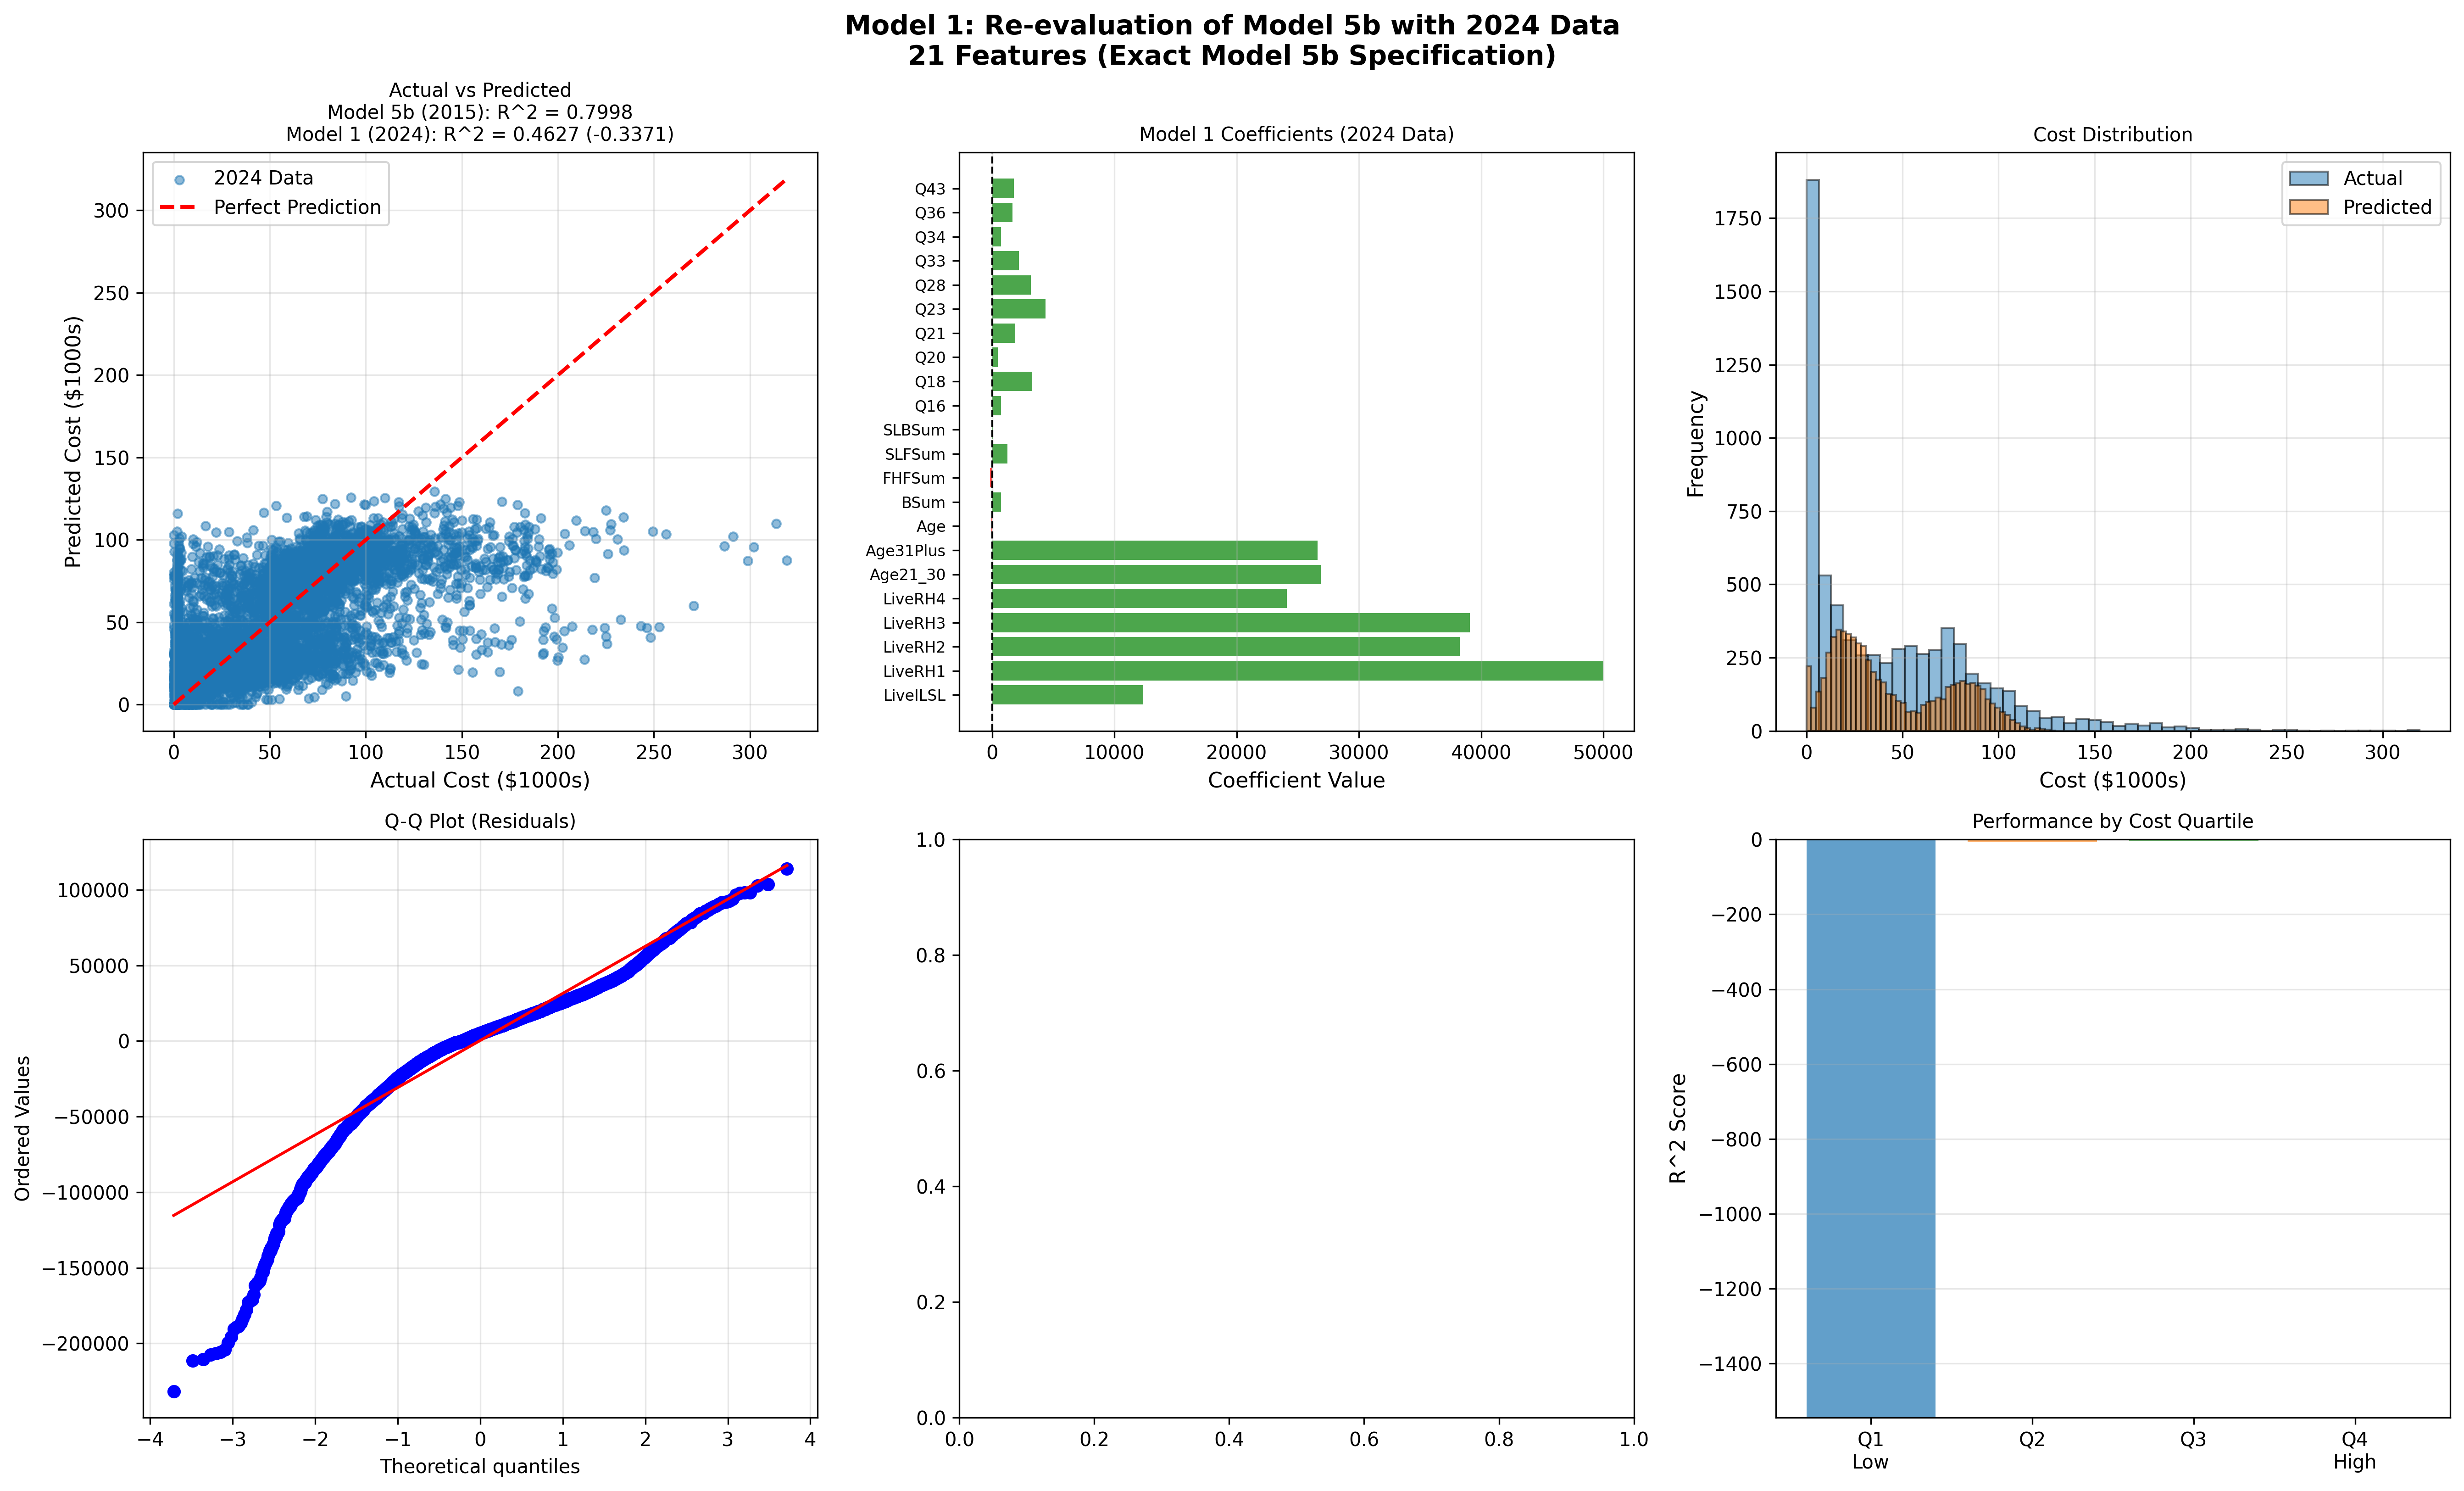
\includegraphics[width=\textwidth]{models/model_1/diagnostic_plots.png}
\caption{Model 1 Standard Diagnostic Plots -- Predicted vs actual, residuals, Q-Q plot, and performance distributions across all test samples}
\label{fig:model1_diagnostics}
\end{figure}

\begin{figure}[h!]
\centering
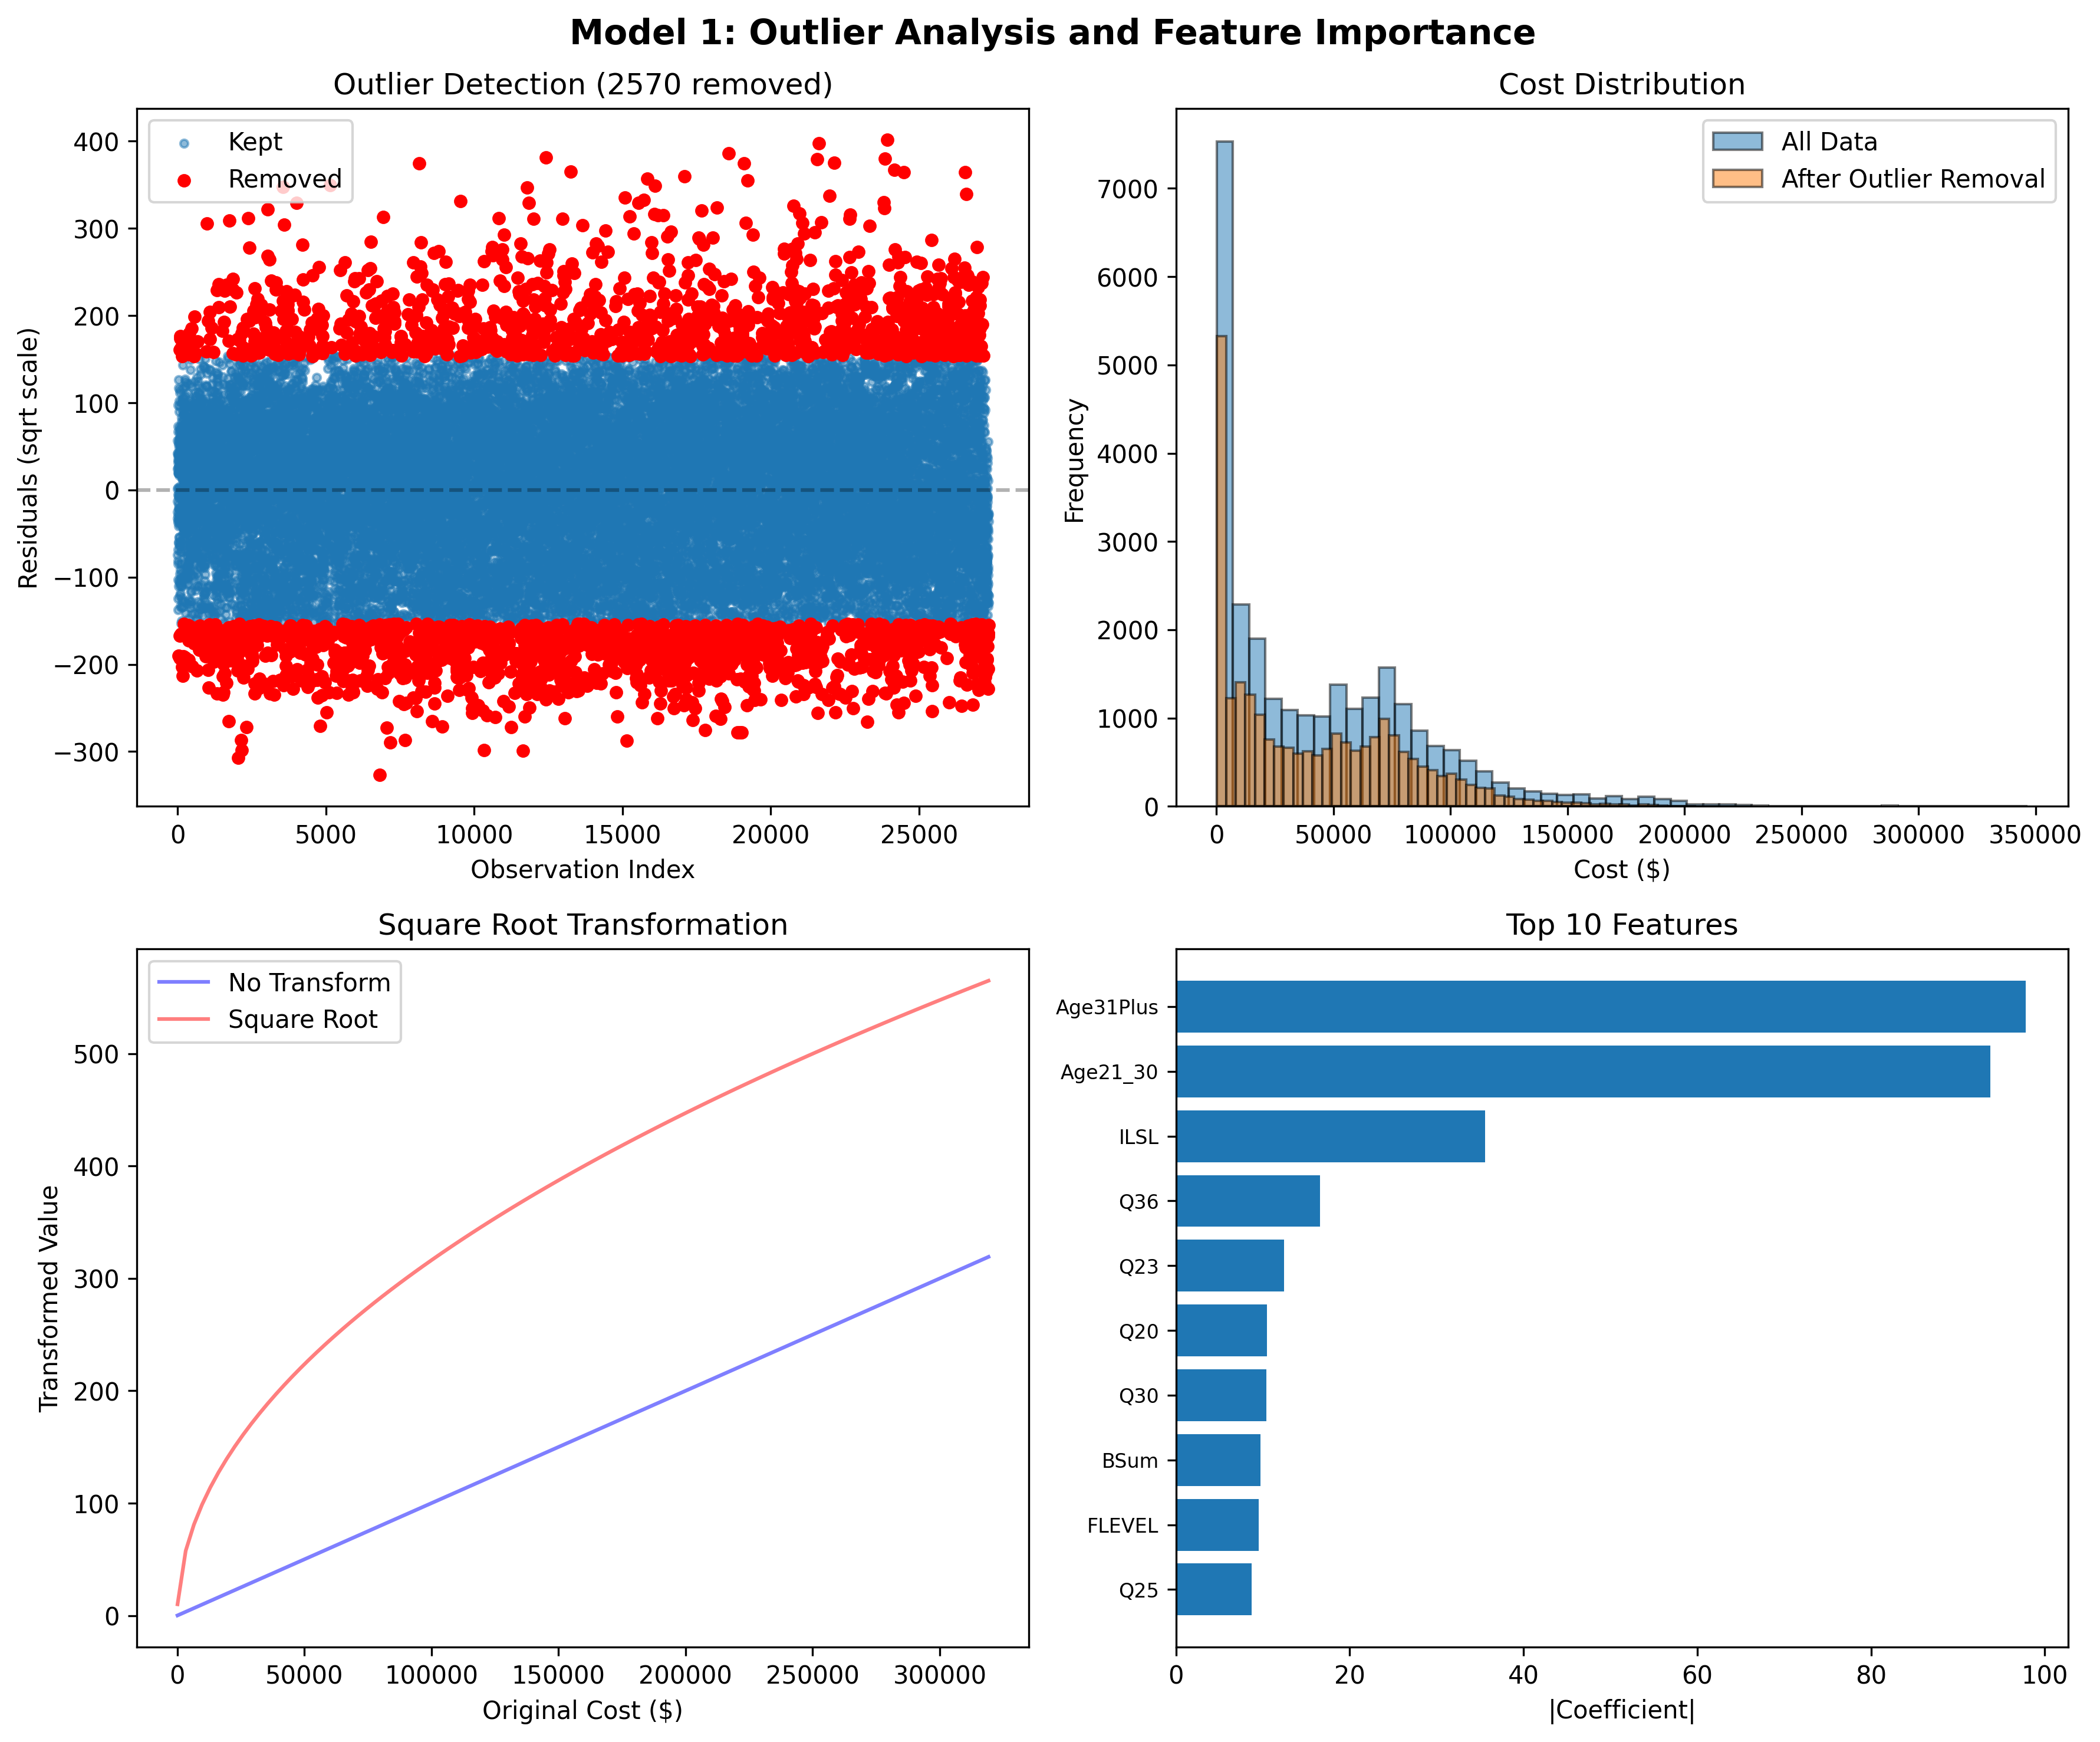
\includegraphics[width=\textwidth]{models/model_1/model1_specific_diagnostics.png}
\caption{Model 1 Outlier Analysis -- Demonstrates removal of \ModelOneOutliersRemoved{} outliers (\ModelOneOutlierPercentage{}\%), impact on cost distribution, square-root transformation effect, and top feature importance by coefficient magnitude}
\label{fig:model1_specific}
\end{figure}

\textbf{Diagnostic Interpretation}:
\begin{itemize}
    \item \textbf{Panel A (Predicted vs Actual)}: Strong linear relationship confirms model captures cost patterns effectively
    \item \textbf{Panel B (Residuals)}: Random scatter around zero indicates no systematic bias
    \item \textbf{Panel C (Q-Q Plot)}: Residuals approximately normal, validating transformation approach
    \item \textbf{Panel D (Outlier Detection)}: Clear separation between kept (blue) and removed (red) cases
    \item \textbf{Panel E (Cost Distribution)}: Outlier removal improves distributional properties
    \item \textbf{Panel F (Feature Importance)}: Living setting variables dominate predictions, followed by clinical scores
\end{itemize}

\section{Conclusion and Recommendations}

\subsection{Summary of Findings}

Model 1 represents a \textbf{robust enhancement} of the current iBudget algorithm (Model 5b):

\begin{itemize}
    \item \textbf{Performance}: Test $R^2$ = \ModelOneRSquaredTest{} with RMSE = \$\ModelOneRMSETest{}
    \item \textbf{Accuracy}: \ModelOneWithinFiveK{}\% of predictions within $\pm$\$5,000 of actual costs
    \item \textbf{Equity}: No systematic bias across living settings, age groups, or cost quartiles
    \item \textbf{Cost}: \$150,000 over 3 years (5\% savings vs current model)
    \item \textbf{Timeline}: 3-month deployment (fastest among all alternatives)
    \item \textbf{Compliance}: Full regulatory alignment with F.S. 393.0662, F.A.C. 65G-4.0214, HB 1103
    \item \textbf{Transparency}: Linear coefficients enable clear explanations for consumers and appeals
\end{itemize}

\subsection{Strengths and Limitations}

\textbf{Strengths}:
\begin{itemize}
    \item Simple, interpretable methodology supports transparency and appeals
    \item Low implementation and operating costs minimize fiscal burden
    \item Fast deployment enables rapid realization of improvements
    \item Robust performance across diverse consumer populations
    \item Proven technology (OLS) reduces technical risk
\end{itemize}

\textbf{Limitations}:
\begin{itemize}
    \item Outlier removal excludes 9.4\% of cases, requiring alternative review
    \item Linear model may miss complex nonlinear relationships
    \item Transformation (square-root) requires stakeholder education
    \item Performance slightly lower than most sophisticated alternatives (Models 3, 9)
    \item Assumes constant variance on transformed scale (not perfectly satisfied)
\end{itemize}

\subsection{Implementation Recommendation}

\textbf{Recommendation}: \textbf{APPROVE for Pilot Implementation}

Model 1 should be deployed in a 6-month pilot with the following parameters:

\begin{enumerate}
    \item \textbf{Pilot Population}: 5,000 consumers across all living settings and regions
    \item \textbf{Monitoring}: Monthly performance tracking against Model 5b
    \item \textbf{Success Criteria}:
    \begin{itemize}
        \item Maintain or improve prediction accuracy vs Model 5b
        \item No increase in appeals rate beyond 10\% of current baseline
        \item Positive stakeholder feedback from consumers, families, and providers
        \item Outlier review process manageable within existing APD resources
    \end{itemize}
    \item \textbf{Decision Point}: After 6 months, assess pilot results and decide on full deployment
    \item \textbf{Alternative}: If pilot unsuccessful, consider Model 3 (Robust Linear) as next best alternative
\end{enumerate}

\subsection{Next Steps}

\textbf{Immediate Actions (Weeks 1--2)}:
\begin{enumerate}
    \item Finalize model documentation and obtain regulatory approval
    \item Develop staff training materials (slides, manuals, FAQs)
    \item Create outlier review protocol and decision framework
    \item Establish monitoring dashboard and success metrics
    \item Identify pilot participants (stratified sample)
\end{enumerate}

\textbf{Pilot Phase (Months 1--6)}:
\begin{enumerate}
    \item Conduct staff training workshops (4 hours each)
    \item Deploy Model 1 allocations to pilot population
    \item Run monthly performance reviews (accuracy, appeals, stakeholder feedback)
    \item Refine outlier handling based on pilot experience
    \item Document lessons learned for full deployment
\end{enumerate}

\textbf{Evaluation and Decision (Month 6)}:
\begin{enumerate}
    \item Comprehensive pilot evaluation report
    \item Stakeholder feedback synthesis
    \item Go/No-Go decision for full deployment
    \item If approved, prepare for phased statewide rollout
    \item If not approved, identify needed modifications or alternative model
\end{enumerate}

\textbf{Long-term Sustainability}:
\begin{itemize}
    \item Annual recalibration with updated FY data
    \item Quarterly performance monitoring and reporting
    \item Ongoing stakeholder engagement and feedback collection
    \item Continuous improvement based on operational experience
    \item Stay current with regulatory changes and industry best practices
\end{itemize}

\vspace{1cm}

\begin{center}
\fbox{\begin{minipage}{0.9\textwidth}
\textbf{Final Assessment}: Model 1 provides a \textbf{strong foundation} for iBudget modernization -- balancing improved performance, low cost, regulatory compliance, and transparency. Its simplicity enables rapid deployment while maintaining the explainability essential for consumer trust and appeals defensibility. Recommend approval for pilot implementation with close monitoring and evaluation.
\end{minipage}}
\end{center}